\documentclass{article}
\usepackage{pgfplots}
\pgfplotsset{compat=1.16} % Adjust to your TikZ/pgfplots version

\begin{document}

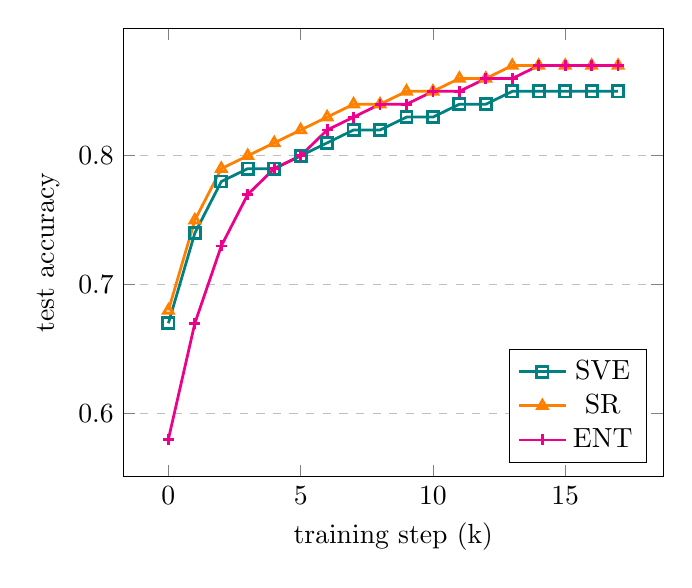
\begin{tikzpicture}
    \begin{axis}[
        xlabel={training step (k)},
        ylabel={test accuracy},
        legend pos=south east,
        ymajorgrids=true,
        grid style=dashed,
    ]
    \addplot[
        color=teal,
        mark=square,
        line width=1pt,
    ]
    coordinates {
        (0,0.67)(1,0.74)(2,0.78)(3,0.79)(4,0.79)(5,0.80)(6,0.81)(7,0.82)(8,0.82)(9,0.83)(10,0.83)(11,0.84)(12,0.84)(13,0.85)(14,0.85)(15,0.85)(16,0.85)(17,0.85)
    };
    \addlegendentry{SVE}
    
    \addplot[
        color=orange,
        mark=triangle,
        line width=1pt,
    ]
    coordinates {
        (0,0.68)(1,0.75)(2,0.79)(3,0.80)(4,0.81)(5,0.82)(6,0.83)(7,0.84)(8,0.84)(9,0.85)(10,0.85)(11,0.86)(12,0.86)(13,0.87)(14,0.87)(15,0.87)(16,0.87)(17,0.87)
    };
    \addlegendentry{SR}
    
    \addplot[
        color=magenta,
        mark=+,
        line width=1pt,
    ]
    coordinates {
        (0,0.58)(1,0.67)(2,0.73)(3,0.77)(4,0.79)(5,0.80)(6,0.82)(7,0.83)(8,0.84)(9,0.84)(10,0.85)(11,0.85)(12,0.86)(13,0.86)(14,0.87)(15,0.87)(16,0.87)(17,0.87)
    };
    \addlegendentry{ENT}
    \end{axis}
\end{tikzpicture}

\end{document}